\chapter{Experimental Results}

\section{Technical Aproach}

In order to evaluate the suitability of advanced light transport algorithms to heterogeneous systems, optimized implementations of all algorithms were developed for both \gls{cpu} and \gls{gpu}. These implementations were developed using specialized ray tracing libraries, namely Nvidia Optix \citep{parker2010optix} and Intel Embree \citep{wald2014embree}.


There are two possible schemes of work decomposition across devices. One is image space decomposition, where each device processes a portion of the image pixels. Another possible alternative is to distribute the algorithm iterations across the devices. In \gls{pt} and \gls{bdpt} the choice between these two approaches is almost irrelevant, however in photon based algorithms (\gls{bpm} and \gls{vcm}) it is not that simple. If image plane division was applied, it would force communication between the \gls{cpu} and the \gls{gpu} in every iteration since the photon map, which would be generated concurrently across the devices, has to be shared among them. If an iteration division was applied, for every \gls{cpu} core a complete photon map would be stored in the main memory.

In order to solve these issues, DICE was configured to consider all the \gls{cpu} cores as a monolithic device, leaving the distribution of work in the \gls{cpu} to the application code. The work between the \gls{cpu} and the \gls{gpu} is then distributed in a set of independent iterations, eliminationg all communication needs. Between the \gls{cpu} cores the image plane is divided, eliminating the excesive memory use. This approach was applied to every developed algorithm in order to ease development and to allow an algorithm independent DICE configuration.

%Integrating both \gls{cpu} and \gls{gpu} implementations using DICE was simple, although some adaptations were applied in order to improve efficiency. DICE considers every \gls{cpu} core as an independant device, the same way it considers a \gls{gpu} for the purpose of work sharing. However, for photon mapping based algorithms this is innapropriate because if image plane division was applied, it would force communication between the \gls{cpu} and the \gls{gpu} in every iteration. If an iteration division was applied, for every \gls{cpu} core a complete photon map would be stored in the main memory. In order to solve these issues, DICE was configured to consider all the \gls{cpu} cores as a monolithic device, leaving the distribution of work in the \gls{cpu} to the application code. The work between the \gls{cpu} and the \gls{gpu} is then distributed in a set of independent iterations, eliminationg all communication needs. Between the \gls{cpu} cores the image plane is divided, eliminating the excesive memory use.



\section{Methodology}

In order to test the scalability and efficiency of the studied algorithms, the execution times of the studied algorithms were measured using only the \gls{gpu}, and while using only the \gls{cpu} or both, with a varying number of \gls{cpu} cores and threads per core, in order to evaluate the gain of using \gls{ht}. Every time measurement was executed five times, selecting the best time as the final result. The workload distribution between the devices was also measured by the DICE scheduler at the end of the five time measurements, being the final result the best possible distribution calculated by DICE. These results represent the fraction of iterations assigned to each device, which may not be a good performance evaluation metric since the iteration time is not uniform, specially in photon mapping based algorithms, in which the iteration time is dependent on the search radius, which decreases in every iteration. These tests were executed using the Living Room Scene with a resolution of 1024x768 and 50 samples per pixel.

In order to evaluate the image quality produced by the studied algorithms, three scenes were used for testing, each with a different goal. The Sponza scene, courtesy of Crytek, is an outdoor scene with only diffuse materials, but complex geometry nonetheless. The Kitchen scene from Lux Renderer, is an indoor scene with glossy materials. The final and most complex scene, the Living Room, courtesy of Iliyan Georgiev, is an indoor scene as well but with an emphasis on reflected caustics and complex lighting. For every scene a reference image was rendered with \gls{vcm} with 100000 samples per pixel. Then for every algorithm a set of images with an approximate rendering time were produced. All these images were compared to the reference image using the \gls{rmse} metric.

\begin{figure}[h]
\centering
\begin{minipage}[b]{0.3\linewidth}
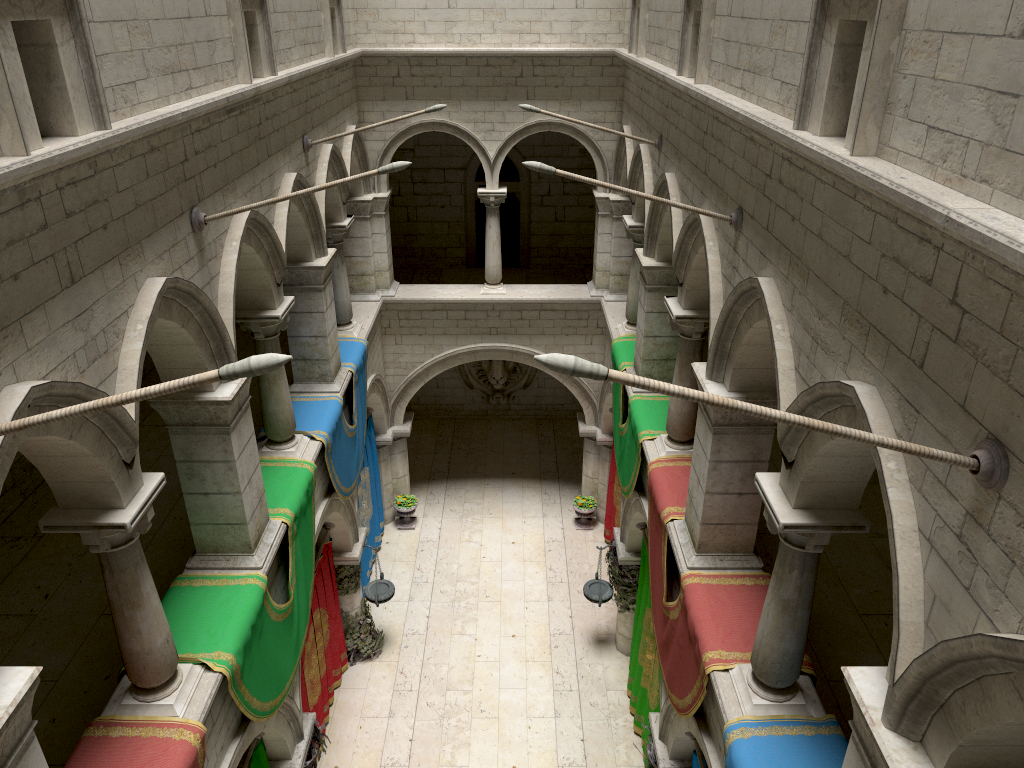
\includegraphics[width=\linewidth]{img/sponza_ref.jpg}
\caption{\label{img:sponza_ref} Sponza scene reference image.}
\end{minipage}
\quad
\begin{minipage}[b]{0.3\linewidth}
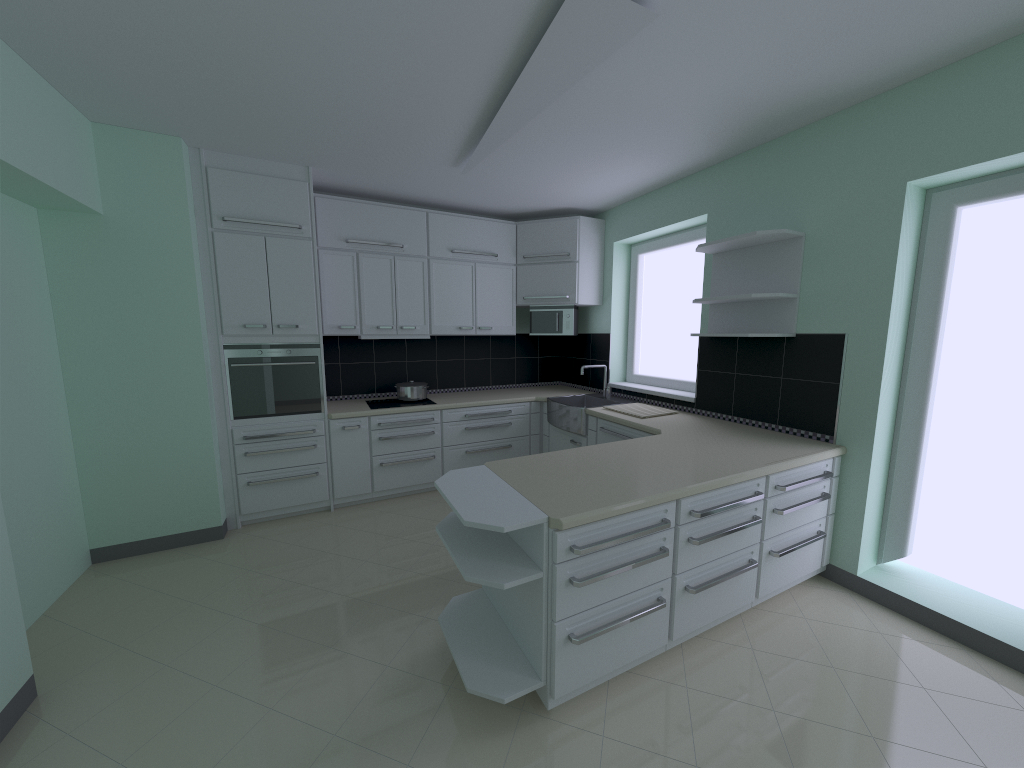
\includegraphics[width=\linewidth]{img/kitchen_ref.jpg}
\caption{\label{img:kitchen_ref} Kitchen scene reference image.}
\end{minipage}
\quad
\begin{minipage}[b]{0.3\linewidth}
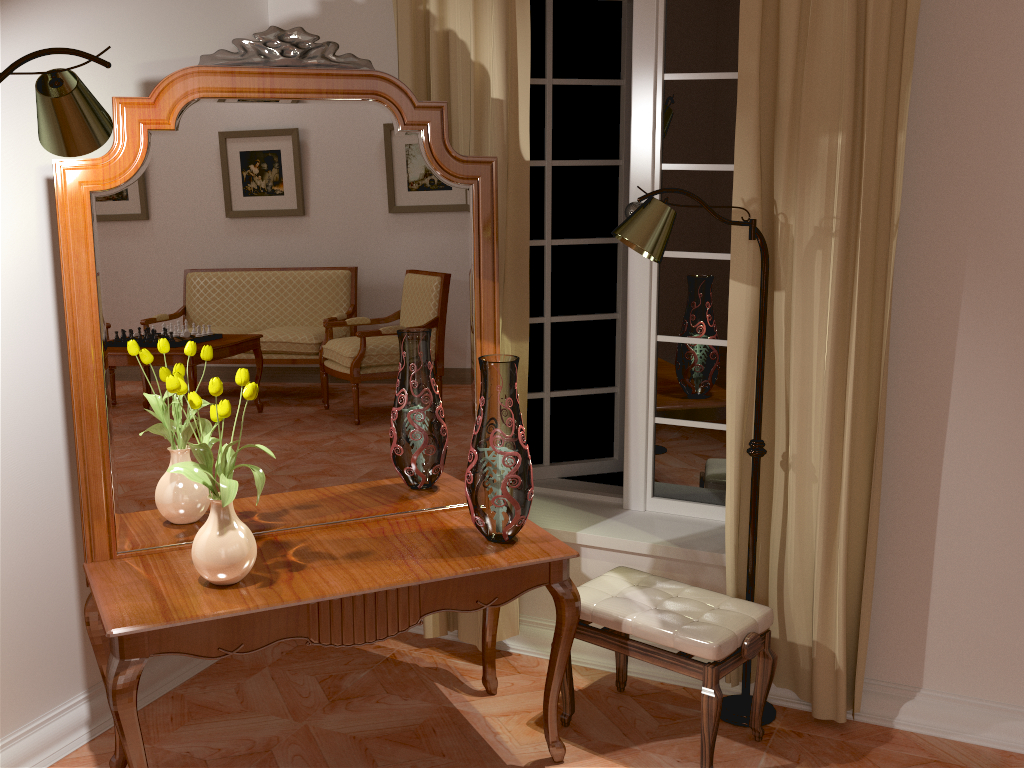
\includegraphics[width=\linewidth]{img/livingroom_ref.jpg}
\caption{\label{img:livingroom_ref} Living Room scene reference image.}
\end{minipage}

\end{figure}

\section{Experimental Setup}

All experiments were executed on a dual-socket computer with two 10 core Intel Xeon E5-2670 v2 \gls{cpu} at the frequency of 2.50GHz, 64 GB of RAM and a Nvidia Tesla K20 \gls{gpu}.

Every software used was updated to the versions listed in table~\ref{tab:soft_ver}.

\begin{table}[h]
\centering
\begin{tabular}{|l|l|}

\hline
Software & Version \\
\hline
Linux & 2.6.32-279 \\
\hline
GCC & 4.8.2 \\
\hline
CUDA Toolkit & 5.5 \\
\hline
Optix & 3.7 \\
\hline
Embree & 2.5.1 \\
\hline

\end{tabular}
\caption{\label{tab:soft_ver} Software Used}
\end{table}

\section{Result Analisys}

\subsection{\label{sec:texec}Excution Time Results}

\begin{figure}[H]
\centering
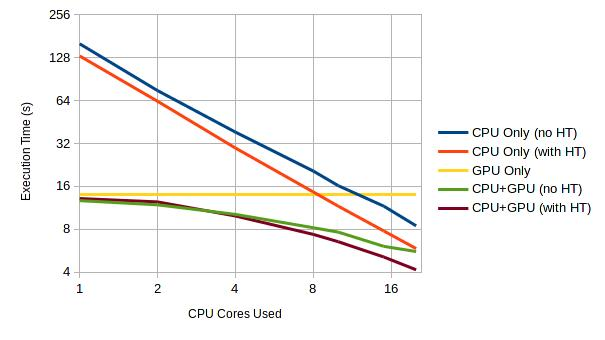
\includegraphics[width=0.8\linewidth]{img/ptTexec.jpg}
\caption{\label{img:ptTexec} Path Tracer Execution Times}
\end{figure}

\begin{figure}[H]
\centering
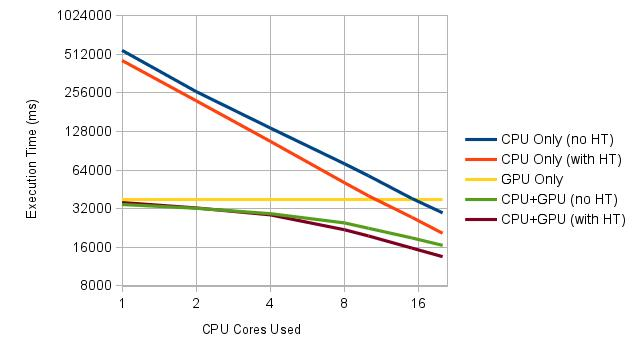
\includegraphics[width=0.8\linewidth]{img/bptTexec.jpg}
\caption{\label{img:bptTexec} Bidirectional Path Tracer Execution Times}
\end{figure}

\begin{figure}[H]
\centering
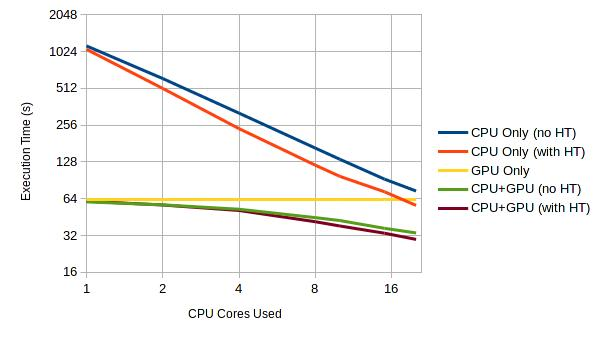
\includegraphics[width=0.8\linewidth]{img/bpmTexec.jpg}
\caption{\label{img:bpmTexec} Bidirectional Photon Mapping Execution Times}
\end{figure}

\begin{figure}[H]
\centering
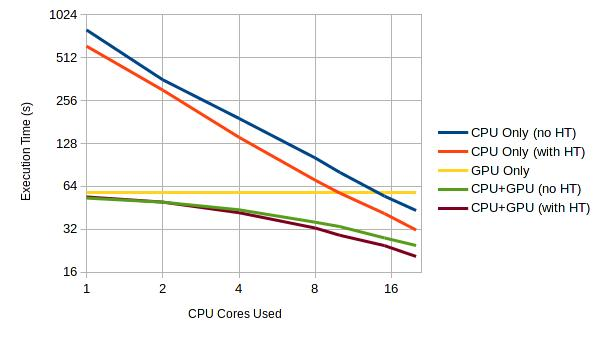
\includegraphics[width=0.8\linewidth]{img/vcmTexec.jpg}
\caption{\label{img:vcmTexec} VCM Execution Times}
\end{figure}

All the execution times measured indicate that all the algorithms studied are scalable and take advantage of both devices in the rendering process. Note that no inflection point was reached, i.e., a point above which execution time starts increasing with additional processing devices. Unfortunately, we were unable to further increase the number of devices in order to detect such inflection point.

\subsection{CPU Speedup Results}

Due to the lack of a clear speedup definition for heterogeneous systems, here is presented only the speedup for the \gls{cpu} implementation. However, in section ~\ref{sec:hefficiency} there is presented an heterogeneous analisys.

\begin{figure}[H]
\centering
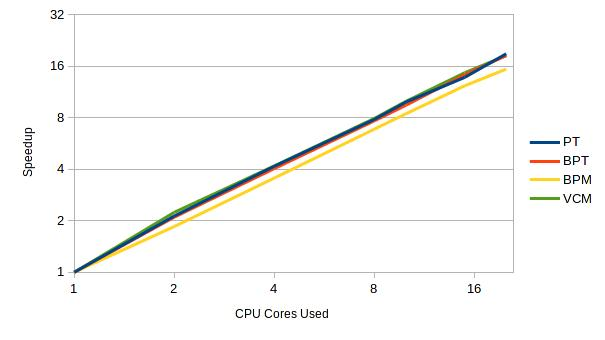
\includegraphics[width=0.8\linewidth]{img/speedup.jpg}
\caption{\label{img:speedup} Speedup Analisys}
\end{figure}

Every algorithm except Bidirectional Photon Mapping achieve an almost linear speedup, while this only achives a speedup of 15.4 using 20 cores. Although not present in this plot, all algorithms seem to take advantage of Hyper Threading, which increases the overall performance between 30\% to 50\%.

\subsection{CPU Parallelization Eficiency Results}

Due to the lack of a clear efficiency definition for heterogeneous systems, here is presented only the efficiency for the \gls{cpu} implementation. However, in section ~\ref{sec:hefficiency} there is presented an heterogeneous analisys.

\begin{figure}[H]
\centering
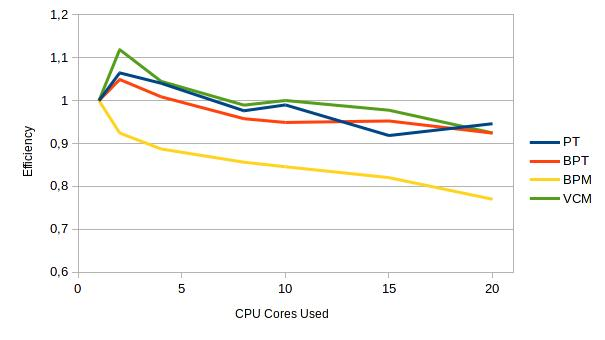
\includegraphics[width=0.8\linewidth]{img/efficiency.jpg}
\caption{\label{img:efficiency} Efficiency Analisys}
\end{figure}

Every algorithms except Bidirectional Photon Mapping has a parallelization efficiency above 0.9, while this falls to an efficiency of 0.77 using 20 cores. This inefficiency may be due to the high memory access this algorithm has compared to all the other algorithms. Note that even though efficiency drops with increased resources, as expected, the inflection point referred in section ~\ref{sec:texec} is still far from being reached.

\subsection{Workload Distribution Results}

\begin{figure}[H]
\centering
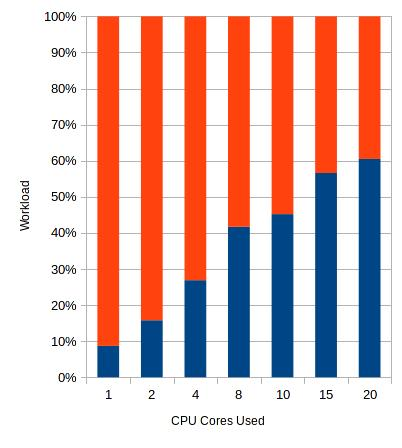
\includegraphics[width=0.8\linewidth]{img/ptwl.jpg}
\caption{\label{img:ptwl} Path Tracer Workload Distribution}
\end{figure}

\begin{figure}[H]
\centering
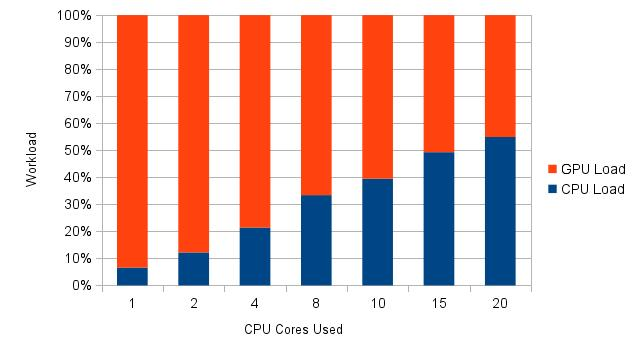
\includegraphics[width=0.8\linewidth]{img/bptwl.jpg}
\caption{\label{img:bptwl} Bidirectional Path Tracer Workload Distribution}
\end{figure}

\begin{figure}[H]
\centering
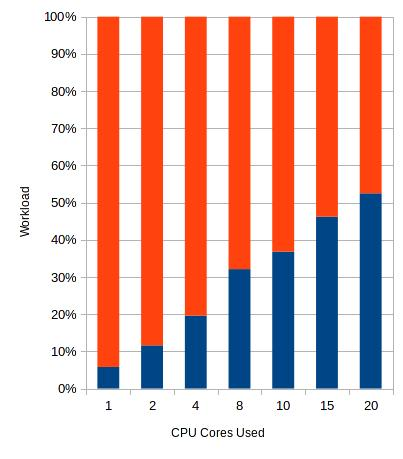
\includegraphics[width=0.8\linewidth]{img/bpmwl.jpg}
\caption{\label{img:bpmwl} Bidirectional Photon Mapping Workload Distribution}
\end{figure}

\begin{figure}[H]
\centering
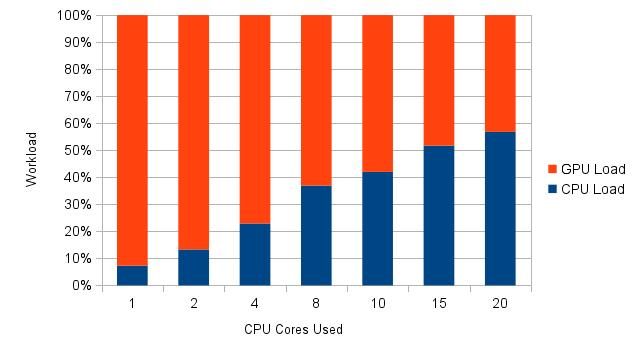
\includegraphics[width=0.8\linewidth]{img/vcmwl.jpg}
\caption{\label{img:vcmwl} VCM Workload Distribution}
\end{figure}

As had been shown by all previous performance metrics these four figures clearly show that the algorithms are able to scale as the number of CPU cores increases. The relative workload processed by the CPU increases with the number of cores, demonstrating that all devices are being used. This behaviour is true and similar for all the four algorithms.

\subsection{\label{sec:hefficiency} Heterogeneous Efficiency}

Although all previous metrics seem to indicate that the tested algorithms use all the resources efficiently, there was no absolute measurement of how well the resources were used.

\cite{Chamberlain98} defined heterogeneous speedup according to equation ~\ref{eq:HetSpeedUp}, where $T_{\mbox{\tiny ref}}$ is the execution time on a reference device selected according to some criterium and $T_D$ is the execution time on an hetereogeneous system constituted by the set $D$ of devices.

\begin{equation}
S_h(D) = \frac{T_{\mbox{\tiny ref}}}{T_D}
\label{eq:HetSpeedUp}
\end{equation}

The optimal heterogeneous speedup, $S_h^*(D)$, can not be defined as function of the number of used devices, because different devices offer different amounts of computational power. \cite{Chamberlain98} expressed this ideal speedup as a ratio of computing rates. 

Let the computing rate for the device $d \in D$ for a given workload $W$ be $R_d = \frac{W}{T_d}$, then the ideal computing rate is the sum of all the computing rates of all the devices $d \in D$.

\begin{equation}
R^*_D = \sum_{d \in D} R_d = W \sum_{d \in D} \frac{1}{T_d}
\label{eq:StarCapacity}
\end{equation}

\cite{Chamberlain98} define $S_h^*(D)$ as the ratio between available computing rate and the computing rate of the reference device:

\begin{equation}
S^*_h(D) = \frac{R^*_D}{R_{\mbox{\tiny ref}}} = T_{\mbox{\tiny ref}} \sum_{d \in D} \frac{1}{T_d}
\label{eq:StarHetSpeedUp}
\end{equation}

Given the definitions of heterogeneous speedup and optimal heterogeneous speedup (equations \ref{eq:HetSpeedUp} and \ref{eq:StarHetSpeedUp}), heterogeneous efficiency can thus be defined as the ratio of both

\begin{equation}
E_h(D) = \frac{S_h(D)}{S_h^*(D)} = \frac{R_D}{R^*_D} = \frac{\frac{1}{T_D}}{\sum_{d \in D} \frac{1}{T_d}}
\label{eq:HetEff}
\end{equation}

Given these definitions, it is possible to calculate the efficiency of the heterogeneous implementations using one \gls{gpu} and a varying number of \gls{cpu} cores, as depicted in the figure ~\ref{img:hefficiency}.

\begin{figure}[H]
\centering
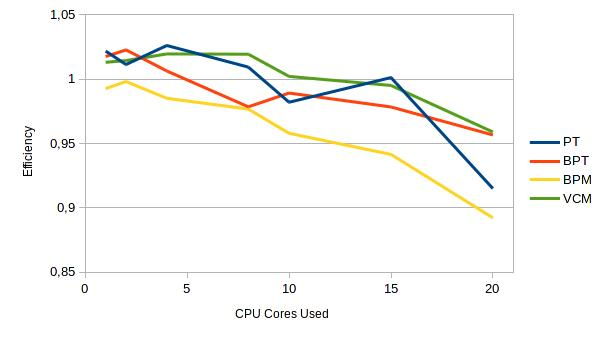
\includegraphics[width=0.8\linewidth]{img/hefficiency.jpg}
\caption{\label{img:hefficiency} Heterogeneous Efficiency Analisys}
\end{figure}

All algorithms achive an heterogeneous efficiency above 0.9, except \gls{bpm}. As with \gls{cpu} efficiency, even though it drops with the increase of resourses, an inflection point is far from being reached.

\subsection{Image Quality Results}

\begin{figure}[H]
\centering
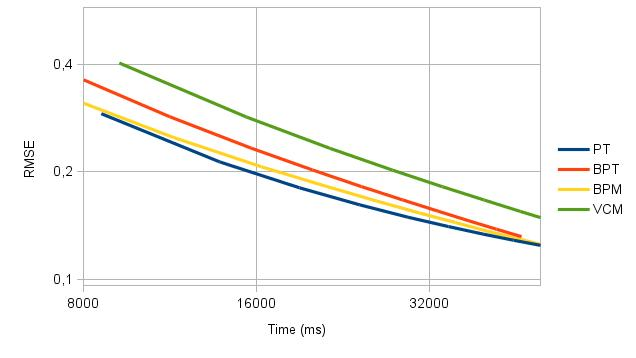
\includegraphics[width=0.8\linewidth]{img/sponzaImgq.jpg}
\caption{\label{img:sponzaImgq} Sponza Image Quality}
\end{figure}

\begin{figure}[H]
\centering
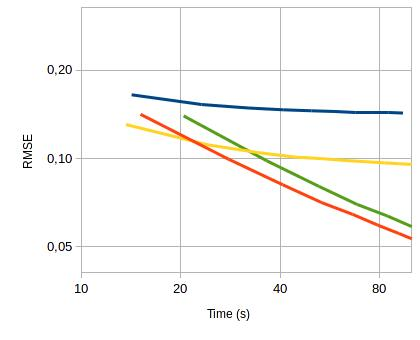
\includegraphics[width=0.8\linewidth]{img/kitchenImgq.jpg}
\caption{\label{img:kitchenImgq} Kitchen Image Quality}
\end{figure}

\begin{figure}[H]
\centering
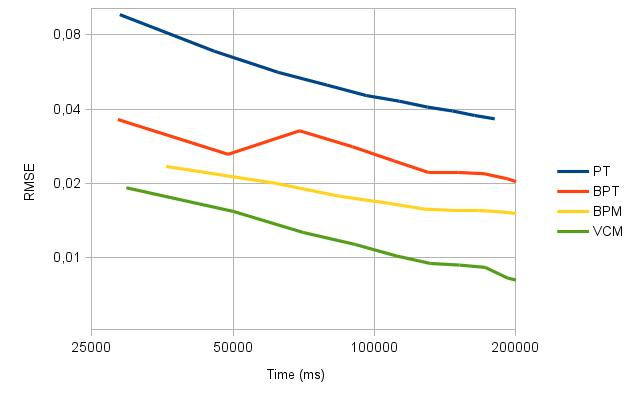
\includegraphics[width=0.8\linewidth]{img/livingroomImgq.jpg}
\caption{\label{img:livingroomImgq} Livingroom Image Quality}
\end{figure}

In the Sponza scene, all algorithms seem to converge to the right solution, however Path Tracing is the best algorithms in this case. This may be due to the outdoor scene configuration where many of the light paths traced are lost and miss the scene, as well as the simple material lighting which is completely captured by Path Tracing, not needing more complex solutions.

In the Kithcen scene, both Bidirectional Path Tracer and Vertex Connecion and Merging algorithms converge to the expected result, although the former is faster for this scene. Both Path tracer and Bidirectional Photon Mapping present lower convergence rates due to the high variance of the lighting effects present, namely caustics incident on glossy surfaces.

In the Living Room scene, Vertex Connection and Merging has the fastest convergence, while the remaining algorithms converges much more slowly. This happened due to the presence of many specular-diffuse-specular paths (namely the reflected caustics in the mirror), which \gls{vcm} was specially designed to capture.